\subsection{Centroiding}

The 3D map can be performed with the coordinates of the light points seen by the camera. They are determined by estimating the center of the spot, and to do so, the center of mass, also called the centroid needs to be calculated in the final image acquired by the color detection. In order to get it, a barycenter of the pixels belonging to the beam is carried out weighted by the intensity of the pixel (S value in HSV model).

\begin{align}
x_c &= \frac{\sum_x x \cdot I(x,y)}{\sum_x \sum_y I(x,y)} \label{xcentroid} \\
y_c &= \frac{\sum_y y \cdot I(x,y)}{\sum_x \sum_y I(x,y)} \label{ycentroid}
\end{align}
Where $x_c$ and $y_c$ are the coordinates of the center of mass of the spot, $x$ and $y$ the coordinates of each pixel belonging to the spot and $I$ their corresponding intensity.

The intensity of each pixel is obtained by splitting the canals of the image into three to retrieve an image with only the Saturation values. Then the formulas \eqref{xcentroid} and \eqref{ycentroid} are computed. A white cross is displayed on the centroid in real time as it can be seen on the figure \ref{fig:finalImage} or below figure \ref{fig:gridCentroiding} on a simple grid image \ref{fig:grid}.

\begin{figure}[!h] 
\centering
\subfigure[Original Image]{
  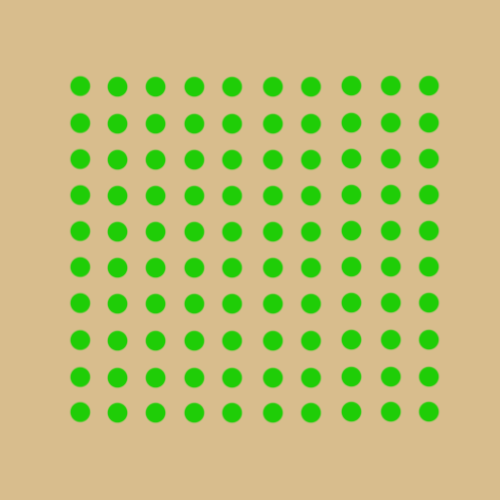
\includegraphics[scale=0.76]{fig/Grid.png}
  \label{fig:grid}
}
\quad 
\subfigure[Final Image with Centroiding]{
  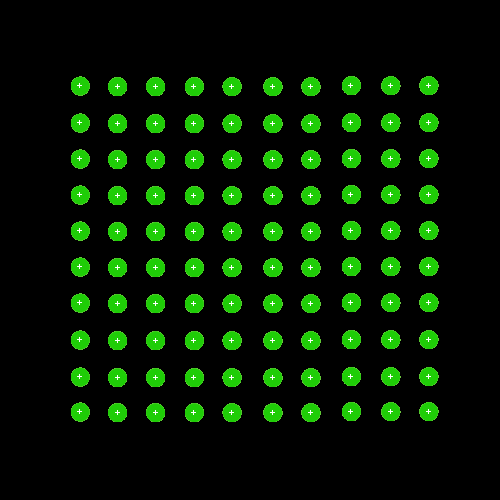
\includegraphics[scale=0.38]{fig/GridCentroiding.png}
  \label{fig:gridCentroiding}
}
\caption{RGB images of a grid of 10 x 10 green points without any noise} 
\end{figure}

In a real application, the grid will not be so perfect after the projection on the rock. Small light spots could be detected as false positive or two points could be slightly linked. In order to deal with these issues, two solutions are implemented. First, during the separation step, if a point has an insignificant number of pixel, it is dismissed. The threshold can be adjusted knowing the expected size of a point. On the other hand, morphological operations (see Theory Section) such as openings are used to disconnect two linked points. The number of erosion and dilation to carry out to separate the points without loosing too much information about the points have to be calibrated. These techniques are tested on the same grid as above, adding some noise (see figures \ref{fig:noisyGrid} and \ref{fig:noisyGridCentroiding}. To make sure that the opening will only slightly change the center of mass of the points, the centroiding method was performed on figure \ref{fig:grid} with and without opening. The coordinates of the centroids were exactly the same in the two cases. The opening has preserved the information. It will be assume that even if there is a slight centroiding error after the opening, it is insignificant.

Several types of noise are added and are denoted figure \ref{fig:noisyGrid}. The first one shows that small changes of green color on a point or inside the same point do not affect the color detection. The second noise is a spot of a green-brown color. As it is expected, it is not detected by the color detection algorithm. Then, the same spot (3 on the figure) but with a color close to the grid points is added to the image. It is detected as a point but its size is under the threshold chosen and it is dismissed as it can be seen on the figure \ref{fig:noisyGridCentroiding}. The opening also ensures that the unexpected spot disappears. The fourth noise represents two linked points. Thanks to the opening, they are well separated on the final image. Finally, the last kind of noise tested (5) is a smaller green spot (which is noise) linked to a real point. The spot is small and even if it is detected by the color algorithm, the opening is efficient enough to delete it. 

\begin{figure}[!h] 
\centering
\subfigure[Original Image]{
  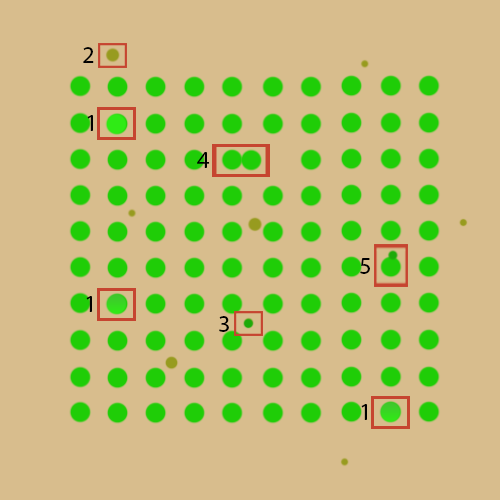
\includegraphics[scale=0.76]{fig/NoisyGrid.png}
  \label{fig:noisyGrid}
}
\quad 
\subfigure[Final Image with Centroiding]{
  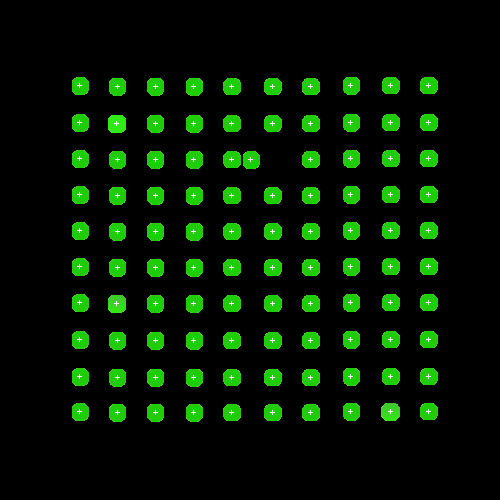
\includegraphics[scale=0.38]{fig/NoisyGridCentroiding.png}
  \label{fig:noisyGridCentroiding}
}
\caption{RGB images of a grid of 10 x 10 green points with noise} 
\end{figure}

It can be concluded that the algorithm is robust enough to handle some noise on computed images. Nevertheless, the deformation and the unexpected light spots or reflets on the rocks could be worse than expected and the algorithm may be incapable of finding the cendroid of each point, with no false positive or false negative. To ensure the robustness of the algorithm, integration tests with a real system have to be carried out.